\documentclass[12pt]{article}

\usepackage[utf8]{inputenc}
\usepackage[T1]{fontenc}
\usepackage[french]{babel}
\usepackage{hyperref}
\usepackage{lastpage}
\usepackage{graphicx}
\usepackage{listings}
\usepackage{subfig}


\begin{document}
\begin{titlepage}
\newcommand{\HRule}{\rule{\linewidth}{0.5mm}}
\setlength{\topmargin}{0in}
\begin{minipage}{0.4\textwidth}
	\begin{flushleft} \large
		\hspace*{-0.5cm}
		\includegraphics[scale=0.20]{./ressources/logo-unicaen.jpg}
	\end{flushleft}
\end{minipage}
\center
\textsc{\large }\\[0.5cm]
\HRule \\[0.4cm]
{ \huge \bfseries Rapport Aide à la résolution de Kakuro}\\[0.4cm]
\HRule \\[1cm]
\begin{minipage}{\textwidth}
	\begin{flushright} \huge
		\center
		Compléments de POO
	\end{flushright}
\end{minipage}\\[1cm]
\textsc{\large }\\[1cm]
\begin{minipage}{\textwidth}
	\begin{flushright} \large
		\center
		PIGNARD Alexandre - 21701890\\BOCAGE Arthur - 21806332
		\\[1cm]
		L3 Informatique - Promotion 2020-2021
	\end{flushright}
\end{minipage}
\textsc{\large }\\[2cm]
{\large \today}\\[0.5cm]
\vfill
\end{titlepage}

\thispagestyle{empty}
\setcounter{page}{0}
\newpage

\tableofcontents
\newpage


\section{Introduction}
Le \textbf{Kakuro} est un jeu logique semblable aux mots croisés. Le jeu est originaire du Jpaon où sa popularité est immense. Le jeu est similaire aux mots fléchés dans lesquels une même combinaison de chiffres ne peut être utilisé deux fois dans la même grille. Bien que le jeu ne soit parvenu en France que vers les années 2004 et 2005 dans le sillage du sudoku, le jeu reste connu depuis longtemps. \\ \\ Source : Wikipedia \\ \\
Le but de ce projet est de créer un logiciel permettant de fournir une aide à la résolution de grilles de kakuro, il ne s'agit pas de proposer une résolution automatique mais de fournir des outils à un joueur afin qu'il résolve de lui même une grille de jeu. \\\ \\
Pour réaliser ce projet, nous avons choisi de le réaliser en Python, langage que nous maitrisions et qui nous offre un large panel de possibilités que cela soit pour réaliser les différentes fonctions dont nous avions besoin mais aussi pour les choix d'interfaces graphiques que nous avions à notre disposition grâce à ce langage. 
\section{Utilisation du programme}
Pour utiliser notre programme, vous pouvez vous rendre dans le répertoire $Kakuro Helper$ et lancer la commande :
\begin{lstlisting}[language=bash]
  $ python3 Main.py
\end{lstlisting}
Afin d'éxecuter le logiciel il faut avoir installé Python 3 sur sa machine ainsi que PyQt5, l'interface graphique que nous avons utilisés. Si ces dépendances sont installées, le logiciel devrait fonctionner sur Linux, Winwows et Mac Os.

\newpage
\section{Conception du programme}
Le projet est divisé en deux grosses paeties, la première est le back-en et se trouve dans le répertoire du même nom. La deuxième est le front-end et se trouve elle aussi dans un répertoire qui porte son nom.
\subsection{Back-end}
Le code présent dans le répertoire back-end constitue le cœur du logiciel. Il correspond aux méthodes qui vont permettre de créer un grille, y associer des valeurs à jouer ou  encore une "heat map". Il s'agit du travail en arrière plan que l'utilisateur ne verra pas et qui sera utilisé par la partie front-end pour interagir avec l'utilisateur.
Le back-end correspond à la partie que l'utilisateur ne verra pas, il s'agit du travail en arrière plan que le front-end va afficher à l'utilisateur. \\ \\ 
Le back-end est constitué de deux sous parties : la partie Logic et les Ressources qui pourront être utilisées. \\ \\
La partie Logic contient les fonctions du logiciel et la partie Ressources contient, comme son nom l'indique, les ressources necessaires au bon fonctionenemtn du back-end (dictionnaire des sommes).
\subsection{Logic}
Dans cette partie nous verrons les différentes fonctions que contient la partie Logic. 
\newpage
Voici un exemple pour illustrer ce travail : 
\begin{figure}[ht]
  \begin{center}
    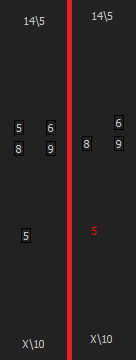
\includegraphics[scale=0.5]{./ressources/retrait.png} 
  \end{center}
  \caption{Avant et après avoir sélectionné le nombre 5 dans une ligne}
\end{figure} 

On voit que lorsque l'on sélectionne le nombre 5, il est retiré des nombres disponibles car il ne peut apparaître qu'une fois dans une ligne. \\ \\
Pour ce qui est de la "heat map" (coloration des cases), elle permet de colorer si on le souhaite les cases qui nous paraissent les plus intéressantes à jouer. Plus la case est foncée, plus elle est intéressante car permettant de débloquer d'autres cases après cette dernière. \\ \\
Enfin, on peut créer sa propre grille via le front-end et le back-end se permettra de la sauvegarder et de la ré-ouvrir si on le souhaite. 
\newpage
\subsection{Front-end}
Le front-end permet l'affichage de la grille et permet à l'utilisateur d'interagir avec le back-end. Il s'agit d'une interface graphique. \\ Cette dernière est réalisée grâce au module PyQt. Le front-end va récupérer les information du back-end et les interpréter et les afficher de manière "lisible" afin que l'utilisateur puisse y avoir accès. \\ \\
Le front-end est divisé en plusieurs fenêtres, la première, celle qui accueille l'utilisateur, permet de sélectionner la grille de kakuro souhaitée. Une fois la grille sélectionnée la fenêtre "helper's side" s'affiche. \\ \\ 
Cette fenêtre est peut-être la plus importante du sujet, elle pemret d'avoir accès aux fonctions du back-end les plus importantes de ce logiciel d'aide à la résolution de kakuro. \\
 \begin{figure}[ht]
  \begin{center}
    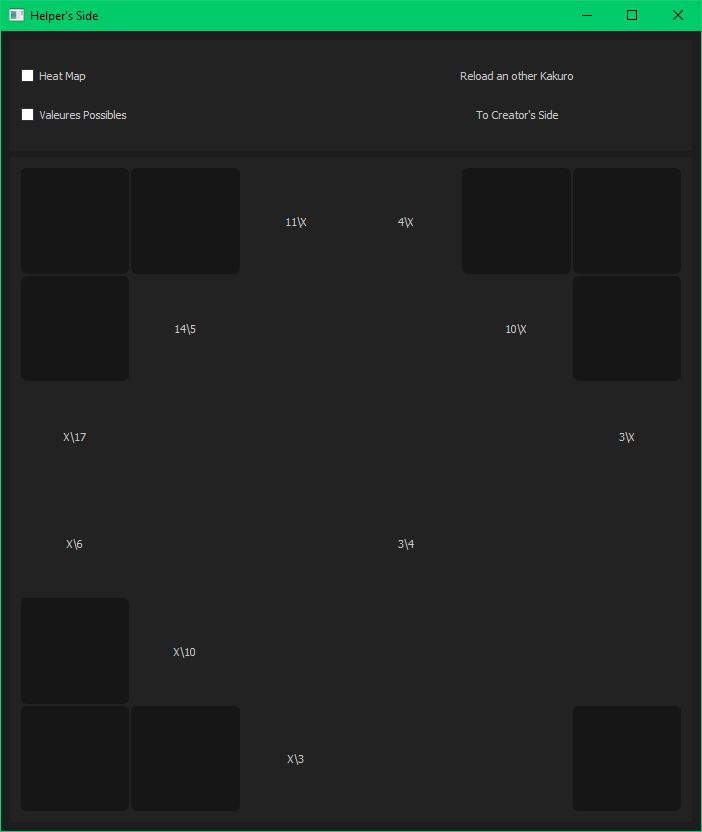
\includegraphics[scale=0.4]{./ressources/helperside.png} 
  \end{center}
  \caption{La grille affichée par l'interface graphique}
\end{figure}

\newpage
Les cases du haut servent à afficher les différentes options disponibles  : la heat map et l'affichage des valeurs possibles. 

\begin{figure}[ht]
  \centering
  \subfloat[Heat map]{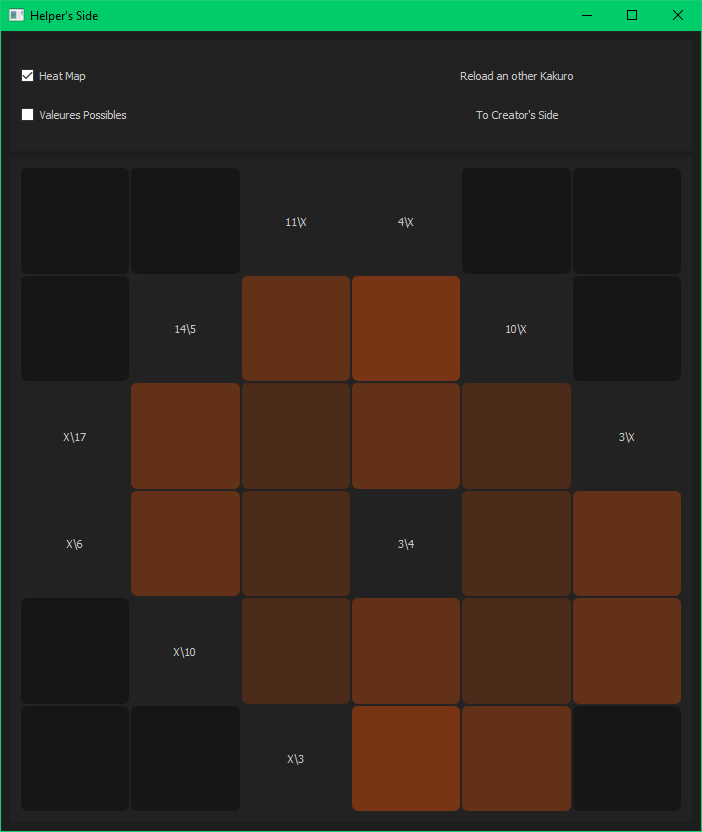
\includegraphics[scale=0.34]{./ressources/heatmap.png}}
  \qquad
  \subfloat[Valeurs possibles]{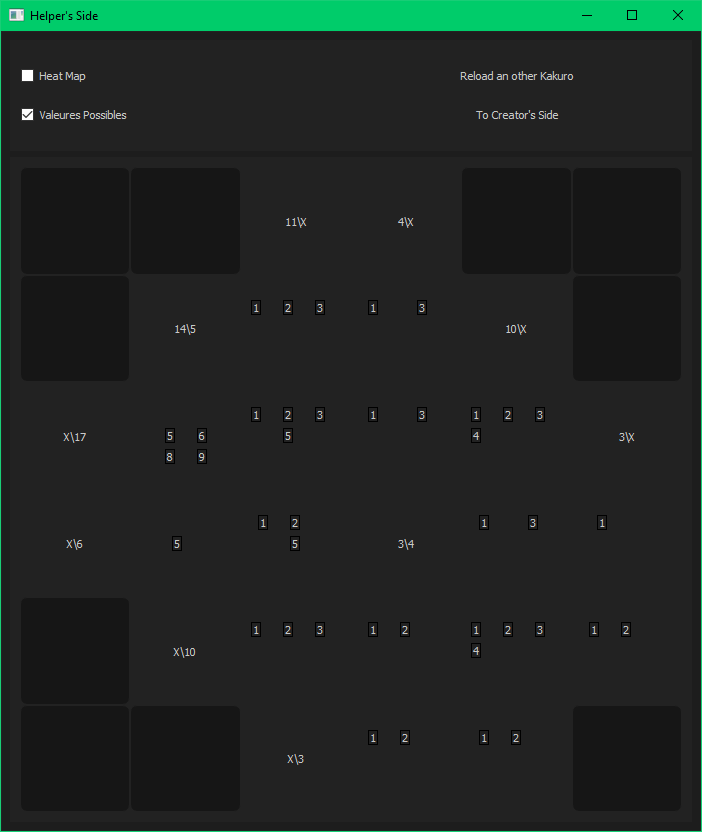
\includegraphics[scale=0.34]{./ressources/valPoss.png}}
  \caption{Exemple des options disponibles}
\end{figure}
\newpage
La dernière fenêtre est celle de création de grille. elle permet de créer sa propre grille si l'on veut utiliser le logiciel pour une grille spécifique. 

 \begin{figure}[ht]
  \begin{center}
    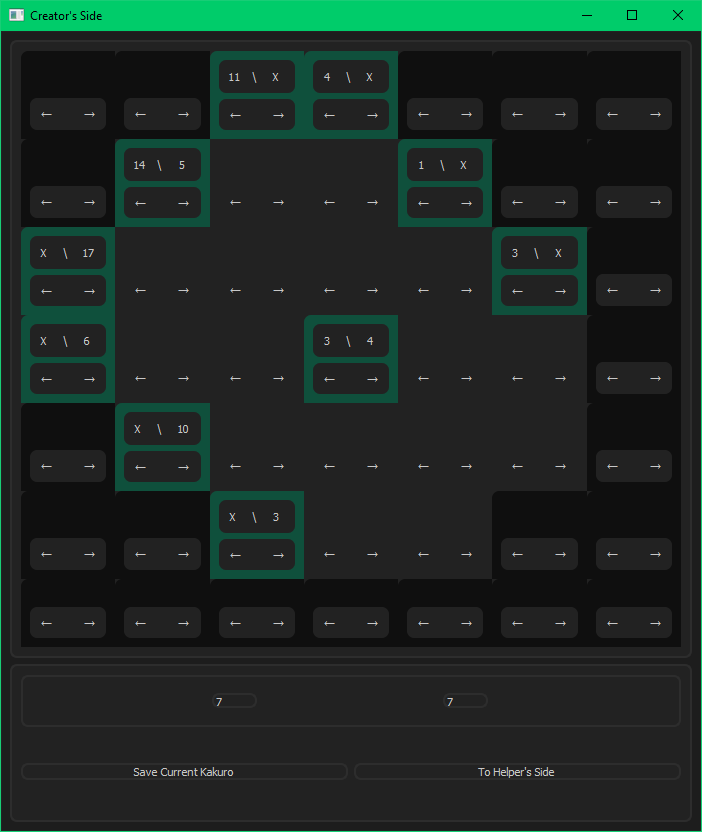
\includegraphics[scale=0.4]{./ressources/creator.png} 
  \end{center}
  \caption{L'outil d'édition de grille}
\end{figure}
Pour ce qui est du style de l'interface graphique, nous avons opté pour un design simple et sombre afin d'avoir un logiciel au visuel épuré et lisible. 
\section{Éventuelles améliorations}
Ce logiciel n'est pas parfait et au vu du temps que nous avions pour le réaliser, nous n'avons pas eu le temps d'y intégrer toutes les options que nous aurions voulu. \\
Par exemple, nous aurions pu mettre un bouton de résolution automatique d'une grille dans le cas où un utilisateur souhaiterai vérifier le bon remplissage d'une grille. \\
\end{document}

